\documentclass[11pt]{article}
\usepackage{amsthm, amsmath}
\usepackage{amsfonts}
\usepackage{xcolor}
\usepackage{graphicx}
\graphicspath{{./img/}}


\newtheorem{definition}{Definition}
\newtheorem{example}{Example}

    \title{Sturm Liouville Problem}
    \author{L}
    \date{July 26, 2022}

\begin{document}
\maketitle

\section{Stum--Liouville Problem}

\textbf{Exercise 3}:

If $\lambda = 0$:
\begin{displaymath}
y = ax+b, y'=a
\end{displaymath}
so, $y(0)-hy'(0)=b-ah=0, \Longrightarrow b = ah$

$y'(1)=a=0, \Longrightarrow a = 0,b=0$, which means $y=0$. So $\lambda=0$ is not an eigenvalue.

If $\lambda <0$:
\begin{gather*}
y=c_1e^{-\sqrt{-\lambda}x} + c_2e^{\sqrt{-\lambda}x} \\
y'=-c_1\sqrt{-\lambda}e^{-\sqrt{-\lambda}x}  + c_2\sqrt{-\lambda}e^{\sqrt{-\lambda}x}
\end{gather*}

Impose the boundary conditions and we get:
\begin{gather*}
y(0)-hy'(0) = c_1+c_2-h(-\sqrt{-\lambda}c_1+\sqrt{-\lambda}c_2)=(1+\sqrt{-\lambda}h)c_1+(1-\sqrt{\lambda}h)c_2=0 \\
y'(1)=-\sqrt{-\lambda}c_1e^{-\sqrt{-\lambda}}+\sqrt{-\lambda}c_2e^{\sqrt{-\lambda}}=0
\end{gather*}
We set the determinant of the systems to zero and get the following equations to solve:
\begin{displaymath}
(1+\sqrt{-\lambda}h)\sqrt{-\lambda}e^{\sqrt{-\lambda}}+(1-\sqrt{-\lambda}h)\sqrt{-\lambda}e^{-\sqrt{-\lambda}}=\sqrt{-\lambda}e^{-\sqrt{-\lambda}}[(1+\sqrt{-\lambda}h)e^{2\sqrt{-\lambda}}+1-\sqrt{-\lambda}h]=0
\end{displaymath}

Since $\lambda \neq 0$, we have to solve \[(1+\sqrt{-\lambda}h)e^{2\sqrt{-\lambda}}+1-\sqrt{-\lambda}h=0 \Longrightarrow e^{2\sqrt{-\lambda}}=\frac{\sqrt{-\lambda}h-1}{1+\sqrt{-\lambda}h}\]

When $h > 1$, there is no solution to this equation. When $0 < h < 1$,there is no solution. When $h=1$, there is no solution.When $h < 0$, there is 1 solution.

If $\lambda > 0$:
\begin{gather*}
y=c_1\cos(\sqrt{\lambda}x)+c_2\sin(\sqrt{\lambda}x) \\
y' = -\sqrt{\lambda}c_1\sin(\sqrt{\lambda}x) + \sqrt{\lambda}c_2\cos{\sqrt{\lambda}x}
\end{gather*}

Impose the boundary conditions and we get:
\begin{gather*}
y(0)-hy'(0)=c_1-h\sqrt{\lambda}c_2=0 \\
y'(1) = -\sqrt{\lambda}c_1\sin{\sqrt{\lambda}} + \sqrt{\lambda}c_2\cos{\sqrt{\lambda}}=0
\end{gather*}

Make some subtitution and we get:\[
c_2\sqrt{\lambda}(-\sqrt{\lambda}h\sin \sqrt{\lambda} + \cos \sqrt{\lambda})=0 \Longrightarrow h\sqrt{\lambda} = \cot \sqrt{\lambda}\]

To summarize:
\begin{enumerate}
\item If $\lambda=0$, we get $y=0$.

\item If $\lambda < 0$, we need to solve the following equation:
\begin{equation}
e^{2\sqrt{-\lambda}}=\frac{\sqrt{-\lambda}h - 1}{1+\sqrt{-\lambda}h}
\end{equation}
which is equivalent to the following with $x>0$
\begin{equation}
e^{2x} = \frac{hx-1}{1+hx}
\end{equation}

\item If $\lambda > 0$, we need to solve the folloing equation:
\begin{equation}
h\sqrt{\lambda}=\cot \sqrt{\lambda}
\end{equation}

which is equivalent to the following with $x>0$ 
\begin{equation}
hx = \cot x
\end{equation}

\end{enumerate}

\begin{figure}
\centerline{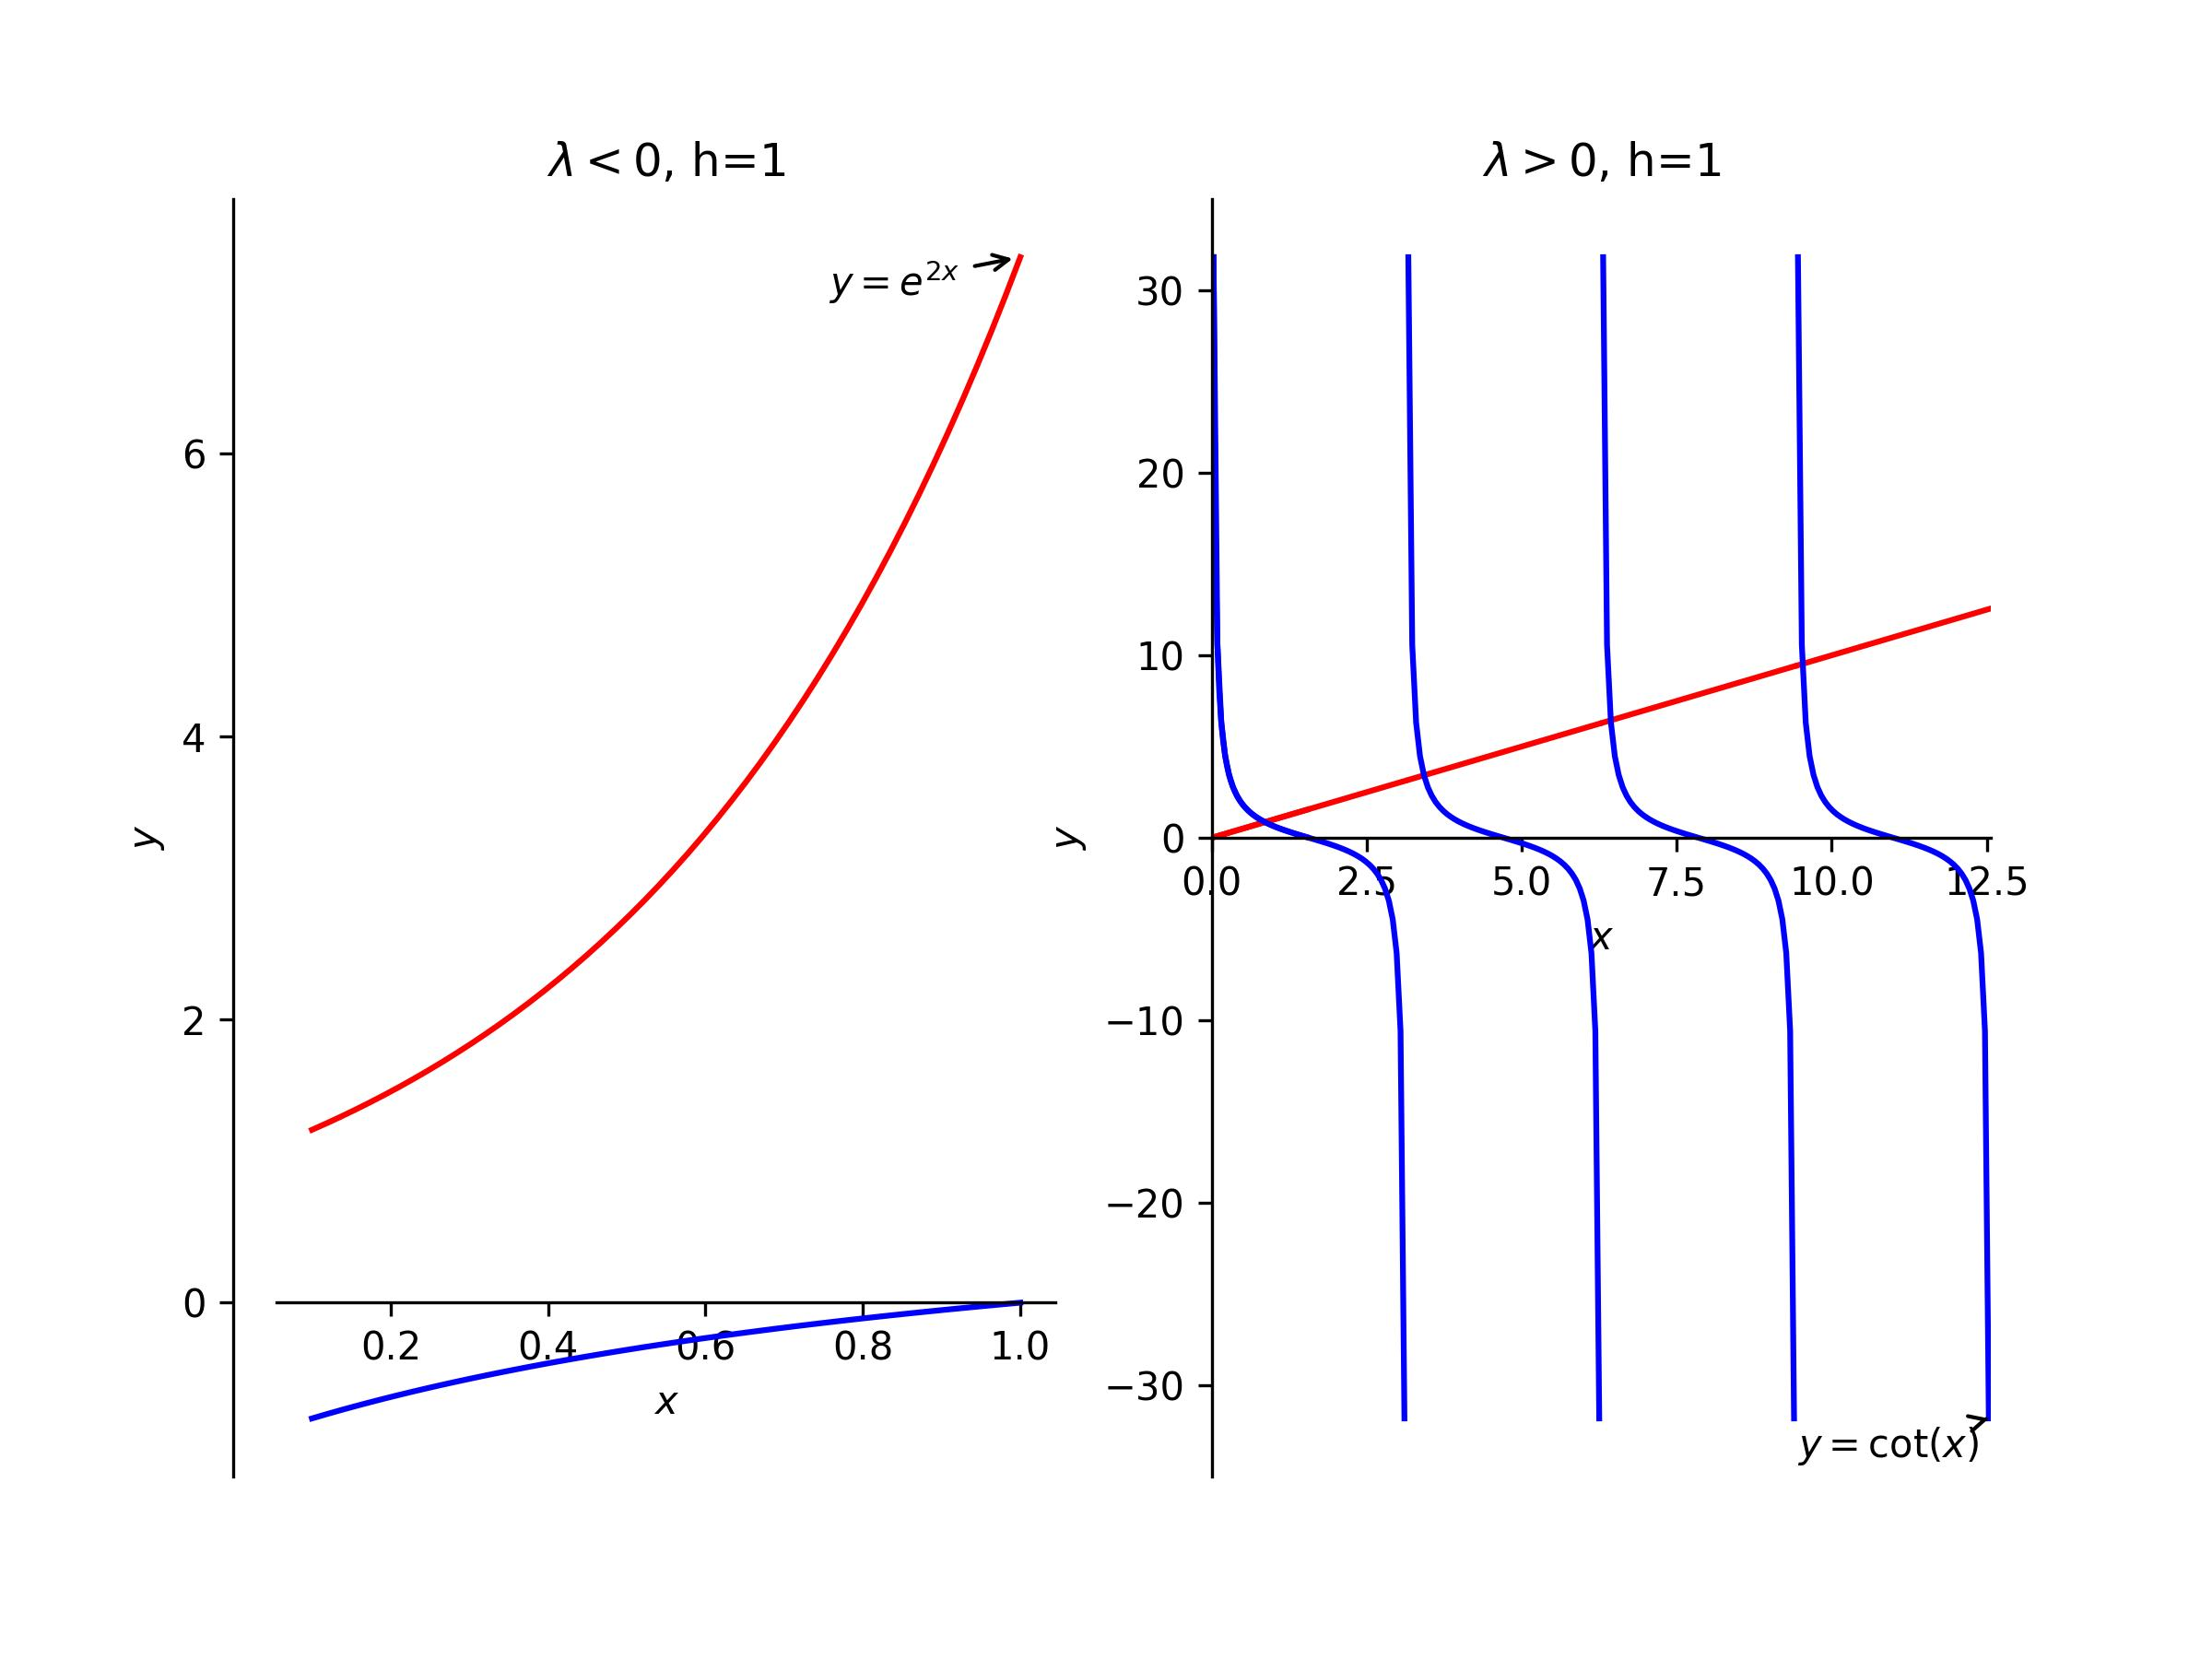
\includegraphics{h_1.jpg}}
\end{figure}


\begin{figure}
\centerline{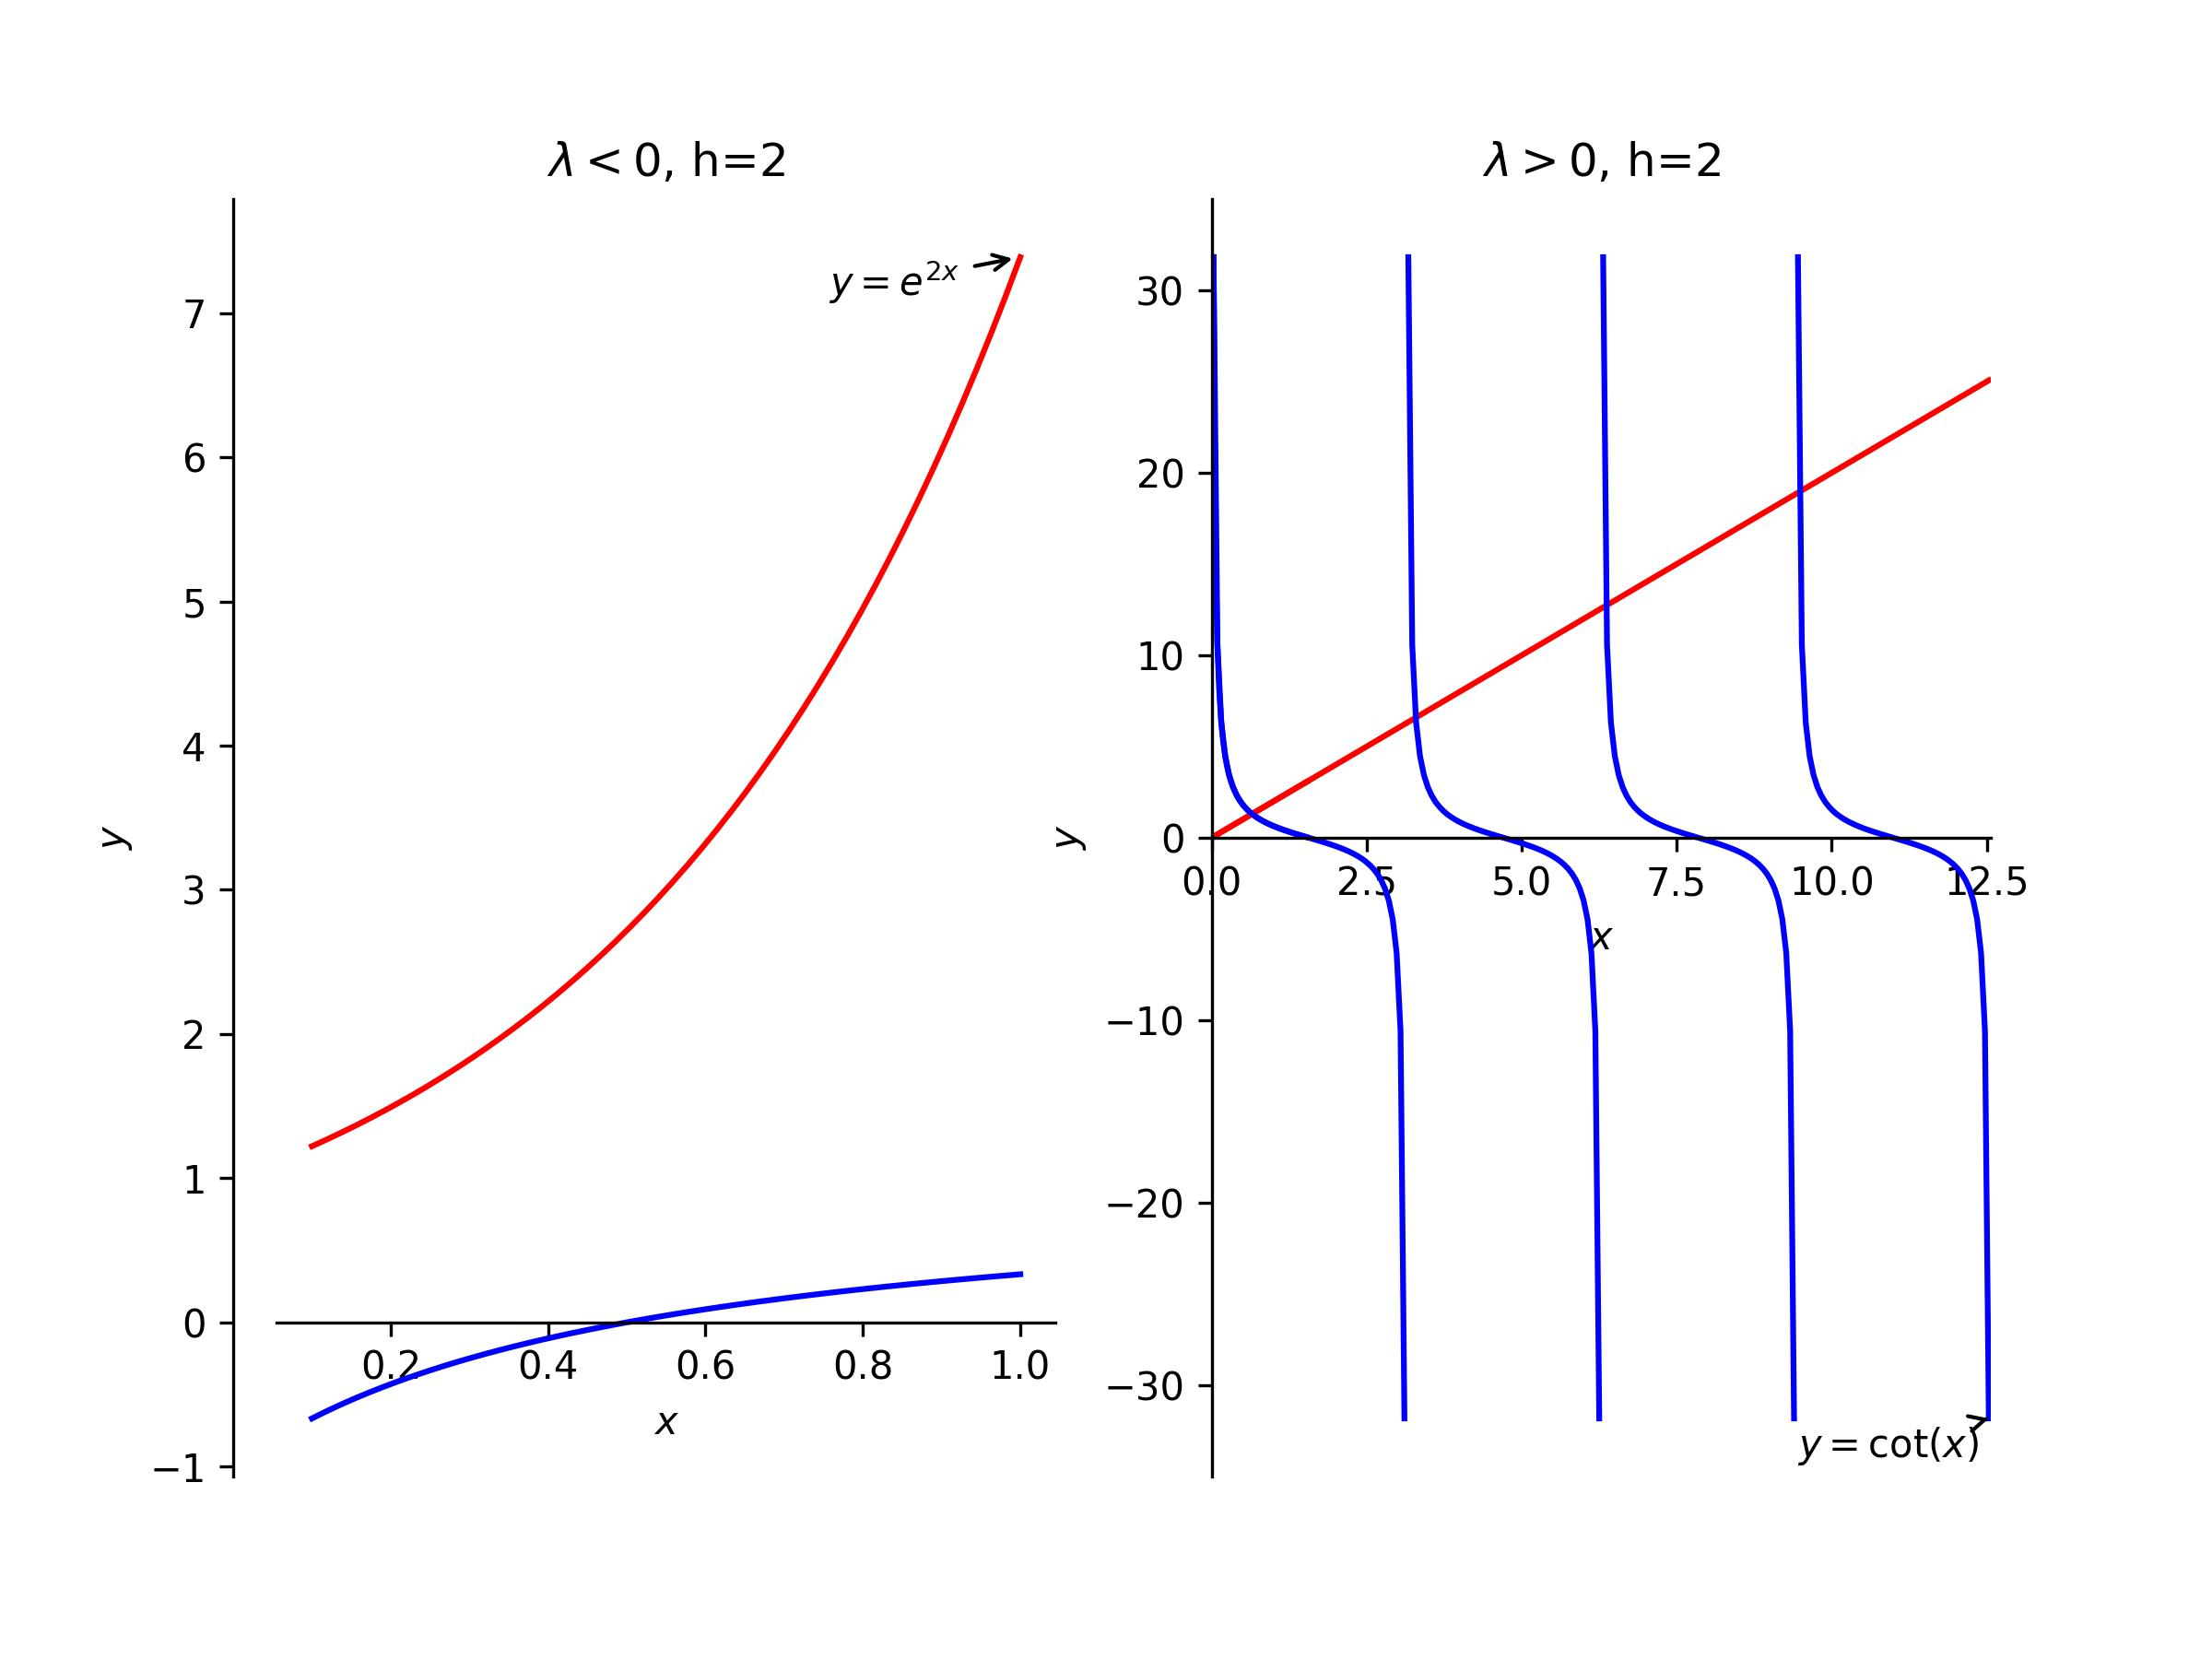
\includegraphics{h_2.jpg}}
\end{figure}

\begin{figure}
\centerline{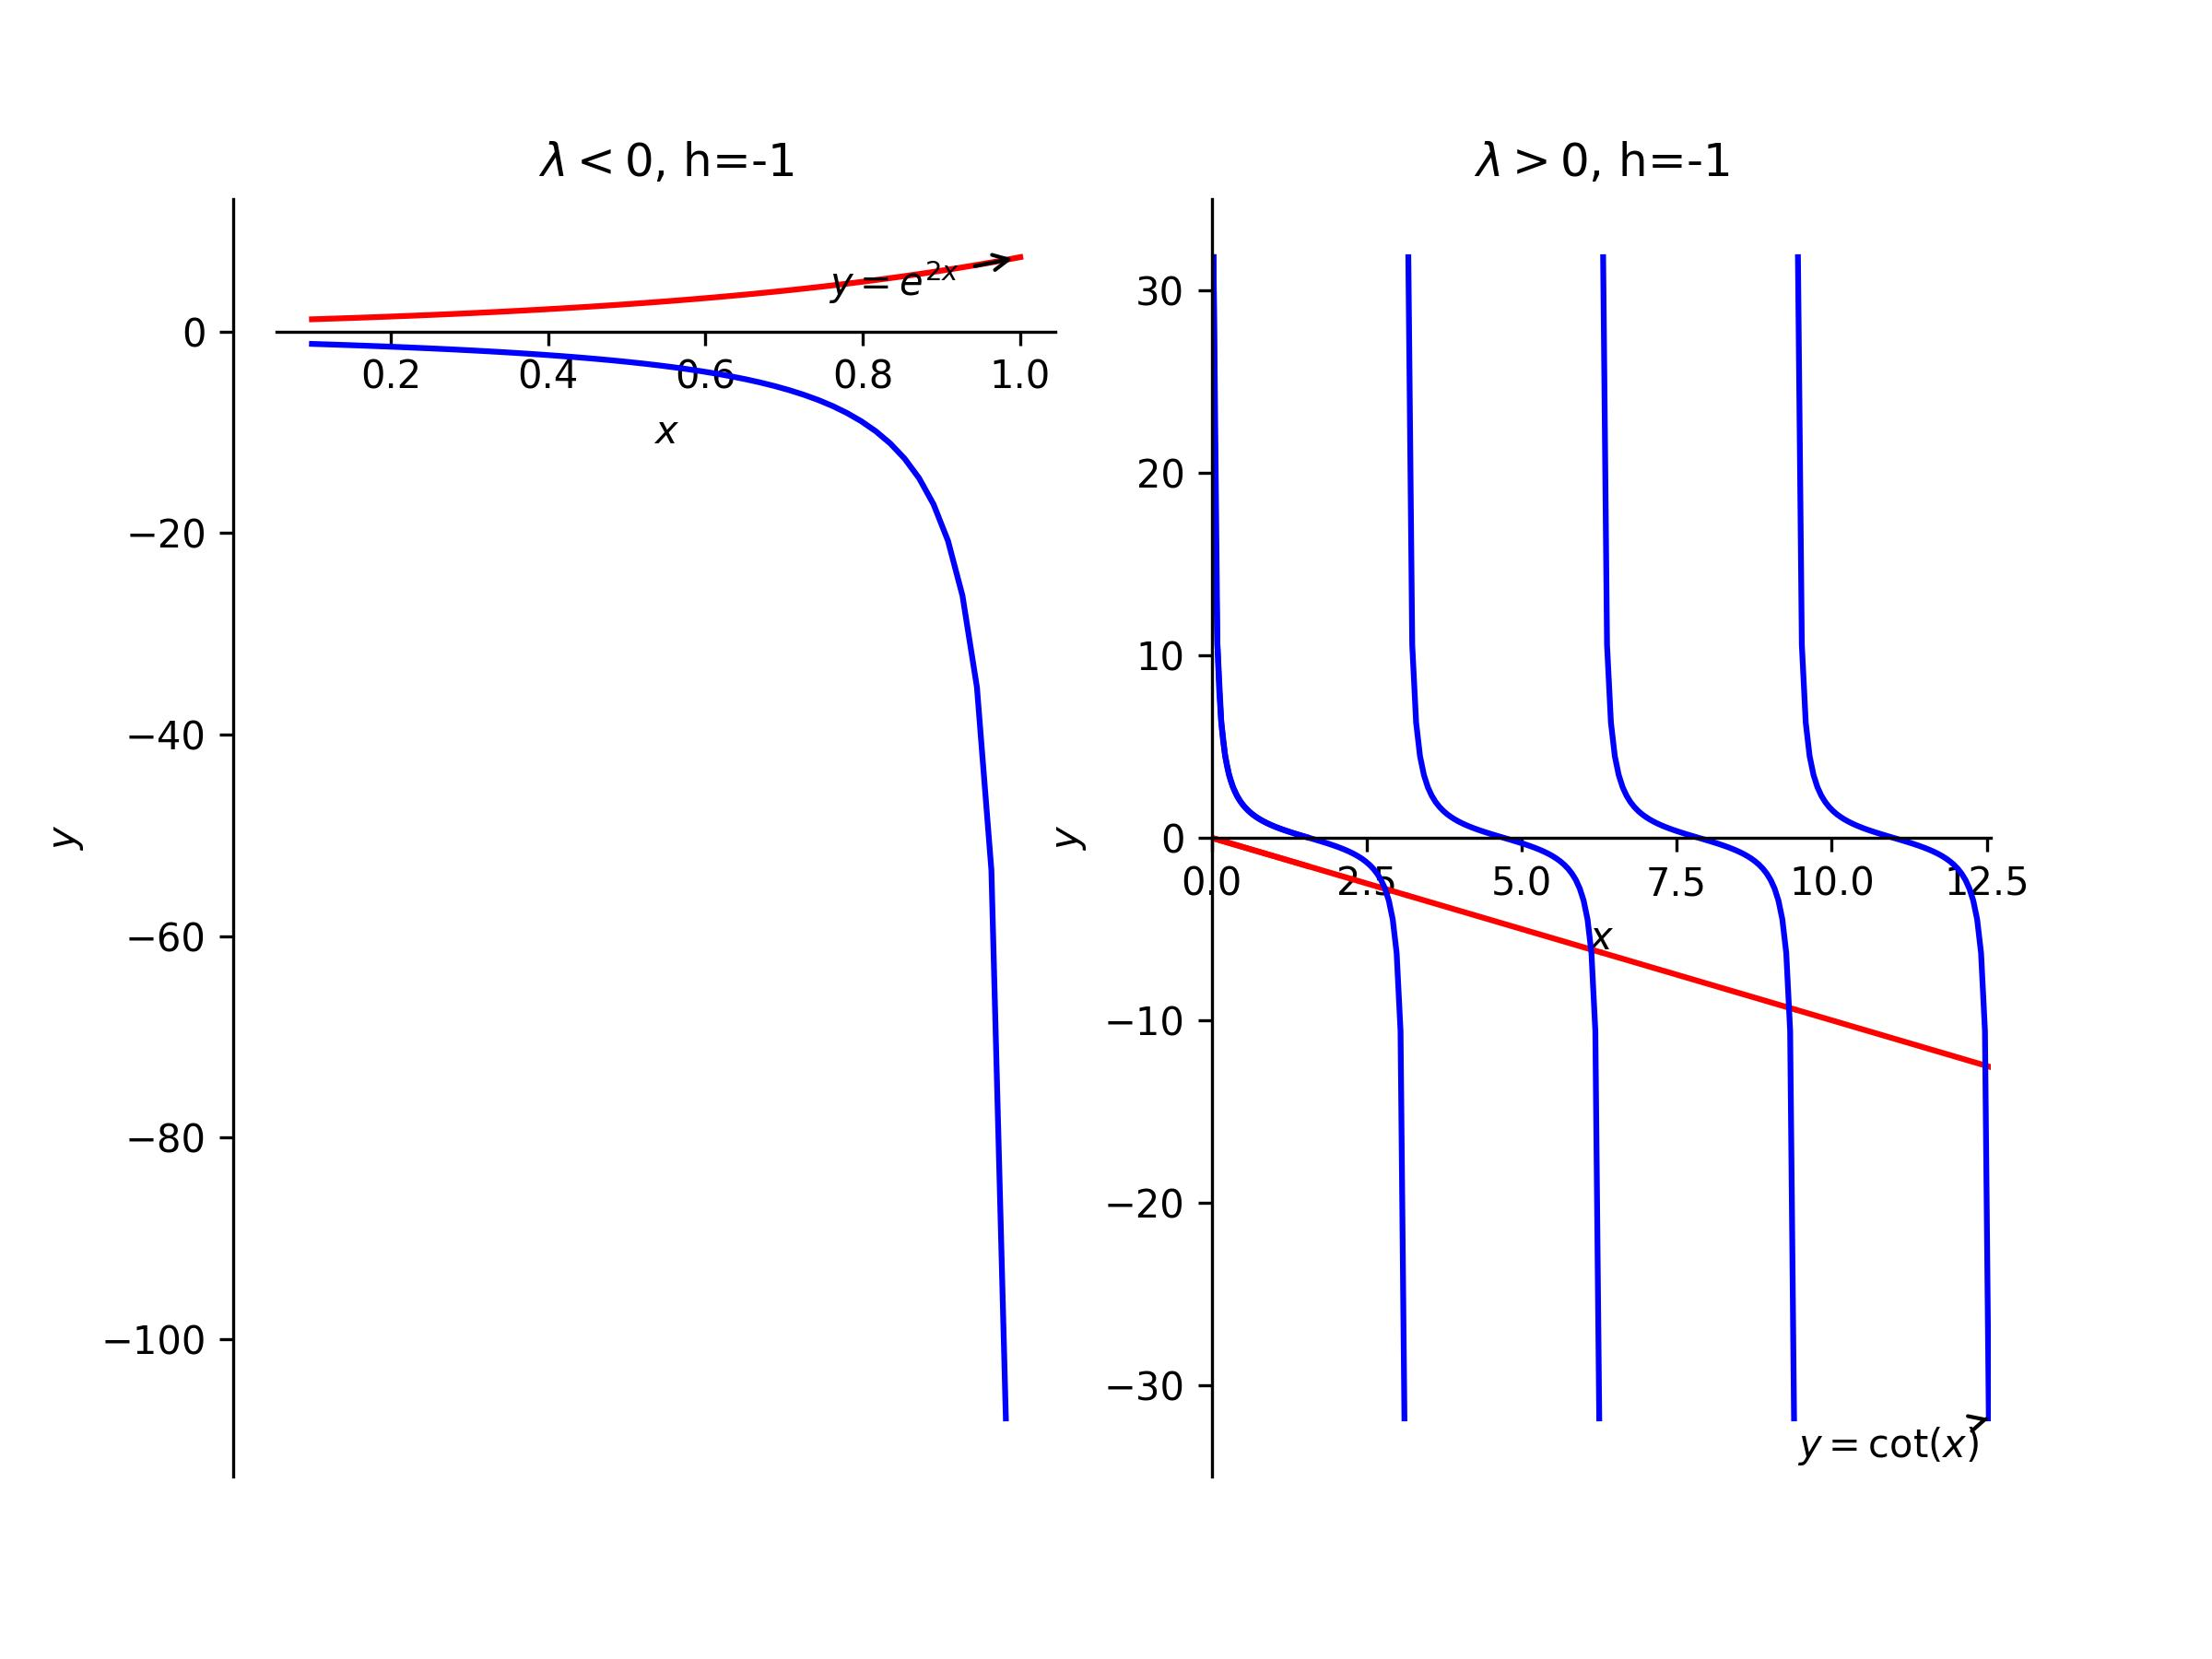
\includegraphics{h_-1.jpg}}
\end{figure}


\end{document}